\documentclass[pra,reprint,superscriptaddress]{revtex4-2}

\usepackage{amssymb,amsthm,bm,mathrsfs,mathtools}
\usepackage[usenames]{xcolor}

\usepackage{graphicx,subcaption}
\graphicspath{{../"img/"}{../"figures/"}}

\usepackage{hyperref}
\hypersetup{
    colorlinks=true,
    citecolor=magenta,
    linkcolor=blue,   
    urlcolor=blue,
}

\bibliographystyle{apsrev4-2}
\def\biblio{\bibliography{references}}


\usepackage{mycommands}
\newcommand{\numcircled}[1]{\raisebox{.5pt}{\textcircled{\raisebox{-.9pt} {#1}}}}
\newcommand{\Dmax}{\trdis_\mathsf{max}}
\newcommand{\InFmax}{\infid_\mathsf{max}}
\newcommand{\Psb}{\mathcal{P}_\mathrm{SB}}
\newcommand{\Odd}{\Omega_{\mathsf{DD}}}
\newcommand{\Opdd}{\Omega_{\mathsf{PDD}}}
\newcommand{\vOpdd}{\vec{\Omega}_{\mathsf{P}}}
\newcommand{\LO}[1]{\operatorname{LO}}
\newcommand{\alphat}{\widetilde{\alpha}}
\newcommand{\betat}{\widetilde{\beta}}

\newcommand{\Ppb}{\mathscr{P}_{\mathrm{0}}}
\newcommand{\Pcp}{\mathscr{P}_{\mathrm{c}}}
\newcommand{\wtP}{\widetilde{P}}
\newcommand{\wtH}{\widetilde{H}}
\newcommand{\wtO}{\widetilde{\Omega}}
\newcommand{\wtU}{\widetilde{U}}
\newcommand{\wt}[1]{\widetilde{#1}}

\newcommand{\HB}{H_\mathrm{B}}
\newcommand{\HSB}{H_\mathrm{SB}}

\newcommand{\Heff}{H_\mathrm{eff}}
\newcommand{\HeffB}{H_\mathrm{eff,B}}
\newcommand{\HeffSB}{H_\mathrm{eff,SB}}

\newcommand{\ep}{\Phi_\mathrm{SB}}
\newcommand{\wtep}{\widetilde{\Phi}_\mathrm{SB}}
\newcommand{\epB}{\Phi_\mathrm{B}}

\newcommand{\CDDn}{\mathrm{CDD}_n}
\newcommand{\rDD}{\mathrm{DD}}
\newcommand{\rmax}{\mathrm{max}}

\begin{document}

\title{Efficacy of noisy dynamical decoupling}
\author{Jiaan Qi}
\affiliation{Yale-NUS College, Singapore}

\author{Xiansong Xu}
\author{Dario Poletti}
\affiliation{Singapore University of Technology and Design}
\author{Hui Khoon Ng}
\affiliation{Yale-NUS College, Singapore}
\affiliation{Centre for Quantum Technologies, National University of Singapore}
\affiliation{MajuLab, International Joint Research Unit UMI 3654,
CNRS-UCA-SU-NUS-NTU, Singapore}


\begin{abstract}
\blue{(To be edited.)}
This paper study dynamical decoupling (DD), a family of pulse schemes aimed at removing noise in quantum systems. We first review the formalism of DD with an emphasis on the error phase, a figure-of-merit characterizing the performance of DD. We then develop noise suppression criteria from the error phase perspective for the periodic and concatenated DD schemes. A rigorous proof for the noise decoupling order of  concatenated DD is also presented.
\end{abstract}

\maketitle




%%%%%%%%%%%%%%%%%%%%%%%%%%%%%
%%%%%%%%%%%%%%%%%%%%%%%%%%%%%
\section{Introduction}
The adverse effects of noise remains the single biggest obstacle to the realisation of large-scale quantum technologies. The very quantum effects that give quantum technologies their edge over classical devices are extremely fragile and easily destroyed by the presence of unwanted interactions with the environment—noise. Much of the current research and technological push in the community today are centered around implementing methods to remove the effects of noise in quantum devices.

A key noise-removal technique is dynamical decoupling (DD)~\cite{viola1999dynamical,duan1998pulse,zanardi1999symmetrizing,khodjasteh2005fault,khodjasteh2007performance,viola2006randomized,uhrig2007keeping,pasini2010optimized,wang2011protection,ng2011combining,kuo2011quadratic}, a low-resource-cost approach that only requires application of fast pulse sequences on individual qubits in the quantum device to average away the effects of noise processes slow compared to the pulse time. With its roots in spin-echo techniques in NMR systems, DD has been used in many different types of experiments as a simple way to reduce noise in quantum information processing systems. Such active noise removal scheme is in direct contrast with the widely studied approach of quantum error correction (QEC)~\cite{Lida2013book}.
Compared with QEC,  dynamical decoupling is typically more economical as it
require no encoding of logical qubits using multiple physical qubits, nor real-time close-loop control through periodic syndrome measurement. All that is needed are regular single-qubit fast pulses that are usually easy to implement. DD be used by itself, or as the first layer of defense against noise In practice, one can choose to only implement DD or to incorporate DD within a standard QEC scheme as the low-level noise-reduction approach. 

The use of DD does not, however, come at no cost. To implement it, one has to apply multiple pulses, which can be imperfect. On the one hand, if the DD pulses are perfect, the slow noise will be averaged away, leaving weaker residual noise on the system; on the other hand, if the DD pulses are imperfect, those imperfections can add errors to the system, and if those errors happen often enough, they can eliminate the benefit of having DD in the first place. Like the cost-benefit analysis familiar to fault-tolerant quantum computing, one has to ask whether there is an error threshold for DD, limiting the level of imperfections allowed in the DD pulses above which DD simply cannot offer any benefit. 

\bigskip
\noindent\blue{More to come.}



\newpage

%%%%%%%%%%%%%%%%%%%%%%%%%%%%%
%%%%%%%%%%%%%%%%%%%%%%%%%%%%%
\section{Preliminaries}
%%%%%%%%%
\subsection{Basics of DD}

DD involves the repeated application of a fixed sequence of short pulses (or fast gates) to individual quantum registers---usually qubits---that averages away the effect of any noise with a time scale slow compared to the sequence time. For a given DD scheme, let $L$ be the number of pulses in the sequence. We denote the $i$th pulse of the sequence as $P_i$, and write the sequence as
$P_L \ldots P_2P_1$ \gray{(I moved the equation here to inline)},
proceeding from right to left in time. Pulse $P_i$ is applied at time $\blue{t_i={} }t_{i-1}+\tau_i$ where $t_{i-1}$ is the time of the application of $P_{i-1}$, and $t_0$ is the start time of the sequence. 
\blue{We illustrate a typcial sequence of DD control gates in \Figref{fig:pulses}. }
\begin{figure}[htbp]
 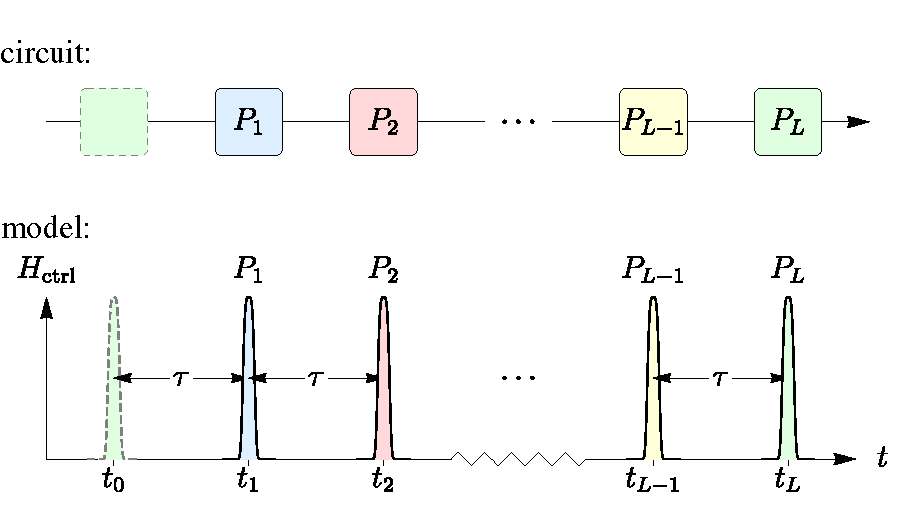
\includegraphics[width=1\linewidth]{pulse.pdf}
 \caption{\blue{Illustration of the external control pulses for a typical DD sequence. Different gates are filled with different colors. The dashed gate at $t_0$ corresponds to the previous DD period.} }
 \label{fig:pulses}
\end{figure}

All DD schemes share some fundamental similarities. First, the pulses are chosen from a specified group of transformations $P_i \in \sG$, for $i=1,2,\ldots, L$.
Second, any DD sequence satisfies the constraint
\begin{equation}\label{eq:fundamental-constraint}
    P_L P_{L-1} \cdots P_1 \stackrel{\textbf{.}}{=} I,
\end{equation}
where the dot above the equal sign means ``up to an overall phase factor". This constraint ensures that there is no net transformation on the quantum register at the completion of the sequence. 
Different strategies could differ in the following aspects:
(i) the transformation group $\sG$.---For a qubit register, an obvious choice is perhaps the Pauli group generated by the Pauli operators $X,Y$, and $Z$. Simpler schemes such as spin echo \cite{Hahn1950} and the CPMG sequence \cite{Carr1954,Meiboom1958} use only the subgroup $\{I,Z\}$.  
(ii) the sequence length $L$ and the specific sequence of pulses.
(iii) the pulse times.---One can have regular-interval pulses, with $\tau_i\equiv \tau$ $\forall i$, as is the case in the periodic DD (PDD) \cite{viola1999dynamical} and concatenated DD (CDD) \cite{khodjasteh2005fault} schemes. One could, however, have variable-interval schemes, such as the Uhrig DD (UDD) sequence \cite{uhrig2007keeping}, nested UDD \cite{wang2011protection}, and quadratic DD \cite{kuo2011quadratic}.
In this work, we focus our analysis on the regular-interval schemes of PDD and CDD, differing in sequence length and the specific pulse sequence, but which both employ pulses drawn from the Pauli group. 

The physical model we are considering is one where gates, including DD pulses, can be applied at some operating frequency, with time $\tau$ in between consecutive gates. A nonzero $\tau$ can be simply the finite switch time between gates, or there may be other practical reasons for a synchronized clock cycle time. We model the DD pulses as instantaneous gates taking no time. There are two sources of errors: (i) the system---the quantum register---interacts with a bath, and that interaction is the source of noise on the system, present even in the absence of the DD pulses; (ii) the pulse imperfections. In past work (see, for example, Ref.~\cite{khodjasteh2005fault}), imperfect DD pulses were modeled as finite-duration pulses during which the alway-on system-bath interaction acts and leads to errors in the pulses. Here, we allow for the more general, and practically relevant, situation of additional control errors in the pulses. We model noisy finite-duration pulses as instantaneous ideal pulses followed by a noise map that captures the background noise as well as any additional control errors. DD sequences are ideally designed to average away the background noise arising from the system-bath interaction. We refer to the original DD sequences with perfect instantaneous pulses as ideal DD, and to the case with imperfect pulses as noisy DD.

In the absence of any DD pulses, the system and bath evolve jointly according to the Hamilton operator $H$, assumed to be time-independent as is appropriate for standard DD analysis (put differently, any parametric time dependence in the joint dynamics occurs because of degrees of freedom excluded from the bath; here we think of all such degrees of freedom as part of the bath). $H$ here can be written as $H=\HB +\HSB$, with $\HB$ as the bath-only Hamilton operator, and $\HSB$ the interaction. No system-only term appears in $H$ as we assume no nontrivial dynamics (other than that arising from $\HSB$) occur in the system during the DD period. With this, we can write the evolution operator for ideal DD as
\begin{equation}\label{eq:Udd}
U_\mathrm{DD}\equiv P_L\upe^{-\upi\tau H}P_{L-1}\ldots P_2\upe^{-\upi\tau H}P_1\upe^{-\upi\tau H}\equiv\upe^{-\upi\Odd}.
\end{equation}
Here, we have defined $\Odd\equiv T\Heff $ as the dimensionless (with the $T$ factor) effective Hamilton operator appropriate for describing evolution for the time of the DD sequence.
$\Odd$ can be written down formally using the Magnus expansion,
\begin{equation}\label{eq:Oeff Magnus series}
\Odd  = \sum_{m=1}^\infty \Odd\up{m},
\end{equation}
where the $m$th term consists of of products of $m$ copies of $\tau H$, and hence of order $\Vert \tau H \Vert^m$. We refer the reader to past analyses of DD \red{(cite)} for a detailed derivation; here we provide only the basic expressions needed for our discussion below. \blue{(Add back a bit of the derivation of the $\Odd^{(1)}$ and $\Odd^{(2)}$ terms.)} Within the radius of convergence of the Magnus series, $\Odd^{(m)}$ decreases in importance as $m$ increases. A DD scheme such that $\Odd^{(m)}$ acts trivially on the system (i.e., acts as $I$ on system) for all $m\leq n$ is said to achieve $n$th-order decoupling---the system sees weakened noise, of strength $\Vert\Odd^{(n)}\Vert\sim\Vert \tau H\Vert^n$, compared to $\Vert\Odd^{(1)}\Vert\sim\Vert \tau H\Vert$ without DD.

\subsection{Quantifying the efficacy of DD}
\blue{(More to come. To put back parts of the fidelity, etc. discussion, as needed in the remainder of the text.)}
\subsubsection{Decoupling Order}


According to \Eqref{eq:formal-Odd}, the DD protocol can be regarded as a transformation $\Omega \to \Odd$. Since the noise map $\cE$ is a function of $\Omega$ and $\rhoB$, the transformation on $\Omega$ takes the original quantum channel into a new 
one  $\cE\to\cE_\sDD$. 
As is argued in Sec.~\!\ref{sec:errph.vs.inf}, error phase is a convenient characterization of noise strength, we apply the two-component norm to the dimensionless Hamiltonian before and after DD, leading to 
\begin{align}
    \opnorm{\Omega} \equiv (\alpha,\beta) \quad \mathrm{and}\quad  \opnorm{\Odd} \equiv (\alpha_\sDD,\beta_\sDD).
\end{align}
The ``decoupling'' reference in the name of DD is understood in terms of the coupling part: i.e., the error phase of the new channel gets reduced through this transformation.
We say noise is suppressed if the ratio $\beta_\sDD/\beta<1$, and a lower ratio would indicate better noise suppression.


A widely used indicator to characterize the performance of DD schemes is the \emph{decoupling order}. A DD scheme is said to achieve $n$th-order decoupling  if the first $n$ terms in the series (\ref{eq:Oeff Magnus series}) have vanishing coupling part:
\begin{equation}\label{dd:nth-order-condition}
\Pcp(\Omega_{\sDD}\up{k}) =0,\ \text{for } 1\le k \le n.  
\end{equation}
The decoupling order is thus a single positive integer to grade different DD schemes. Greater decoupling order is usually linked with better noise suppression rate. 
This can be seen by evaluating the norm of the Magnus series projected on to the coupling part. For an $n$th-order decoupling sequence, we have
\begin{equation}\label{eq:nth-order-alternative}
\beta_\sDD 
=\norm[\Big]{\sum_{ k=n+1}^\infty \!\!\! \Pcp(\Omega_{\sDD}\up{k}) }
\simeq (\alpha,\beta)^{n+1},
\end{equation}
where we use the notation $(\alpha,\beta)^{n+1}$ to represent a polynomial that is $(n+1)$th order in $\alpha$ and $\beta$.
Provided that the Magnus series convergences absolutely, $\beta_\sDD$ is bounded by a power series in $\norm{\Omega}$ whose leading term is on the order of $n+1$.
Therefore \Eqref{eq:nth-order-alternative} provides an alternative characterization for the $n$th-order decoupling condition, which can be useful when directly calculating the first $n$ Magnus terms is unfeasible.




\subsubsection{Error Phase}
To gauge the efficacy of DD, we need to quantify the deviation of the actual state of the quantum system, with and without DD, from the ideal, no-noise state. Following Ref.~\cite{khodjasteh2007performance}, we make use of the \emph{error phase}, which measures the strength of the system-bath interaction, the source of the noise on the system. The system and bath evolve jointly for some specified time $T$ according to the evolution operator $U(0,T)$. The underlying joint Hamilton operator generating the dynamics can be time-dependent, and can include---or not---the DD pulses on the system. We write $U(0,T)\equiv \upe^{-\upi T\Heff}$, for some effective time-independent system-bath Hamilton operator $\Heff$. $\Heff$ can be split into two pieces: $\Heff\equiv \HeffB+\HeffSB$, where $\HeffB\equiv \frac{I_\mathrm{S}}{d_\mathrm{S}}\otimes\tr_S(\Heff)$ acts on the bath alone, while $\HeffSB\equiv \Heff-\HeffB$ contains all the pieces that act nontrivially on the system. $\HeffSB$ can be thought of as the effective system-bath interaction over this time $T$. We define the error phase as the norm of that interaction, multiplied by the time interval,
\begin{equation}\label{eq:ErrorPhase}
\ep\equiv T\Vert\HeffSB\Vert .
\end{equation}
We use a norm such that $\Vert S\otimes B\Vert = \Vert S\Vert \Vert B\Vert$, and $\Vert I\Vert =1=\Vert X\Vert = \Vert Y \Vert =\Vert Z\Vert$ for single-qubit $I, X, Y$, and $Z$.

As we will see, the norm of $\HeffB$ will also enter our analysis. We define the corresponding error phase for the bath-only term as $\epB\equiv \Vert\HeffB\Vert T$, and also ``two-component" error phase as
\begin{equation}
\Phi\equiv T\opnorm{\Heff}\equiv (\epB,\ep)
\end{equation}
\blue{(To merge with new text.) }\gray{
Following the properties of operator norm, thus-defined map is  absolutely-scalable $\opnorm{a\, \Omega}= |a|\cdot \opnorm{\Omega}, \forall a \in \mathbb{C}$,
and satisfies the inequality, 
$\opnorm{A+B}\le \opnorm{A} + \opnorm{B}$,
where  the ``$\le$'' sign between number pairs  is defined by each of the components: $(a_1,b_1)\le(a_2,b_2)$ if both $a_1\le a_2$ and $b_1\le b_2$; vice versa for  the ``$\ge$'' sign. 
It can also be easily verified that the two-component norm is invariant under arbitrary disjoint unitary transformation on $\cH_\rS\otimes\cH_\rB$:
\begin{equation}
    \opnorm{(U_\rS \otimes U_\rB) \Omega (U_\rS ^\dagger \otimes U_\rB)} = \opnorm{\Omega},\, \forall U_{\rS} (U_{\rB})  \in \sU(d_{\rS(\rB)}),
\end{equation}
where $\sU(d_{\rS(\rB)})$ is set of unitary operators on $\cH_\rS$ or $\cH_\rB$.
This invariance suggests that the error phase is invariant under arbitrary interaction picture defined by a system or bath evolution.
}

\subsubsection{Channel fidelity measures}

\subsection{PDD and its concatenation}
We specialize here to the case of interest, that of the single-qubit PDD scheme. The single qubit interacts with a bath, with a joint Hamilton operator (in the absence of DD) that can be written, without loss of generality, as
\begin{equation}
H\equiv I\otimes B_I+X\otimes B_X+Y\otimes B_Y+Z\otimes B_Z,
\end{equation}
where $I$ is the identity operator on the qubit, $X,Y$, and $Z$ are the Pauli operators on the qubit, and $B_i$, for $i=I,X,Y,Z$, are operators on the bath. We identify $I\otimes B_I$ as the bath-only $H_\mathrm{B}$ and $X\otimes B_X+Y\otimes B_Y+Z\otimes B_Z$ as the interaction Hamilton operator $H_\mathrm{SB}$, and define
\begin{equation}
\opnorm{\tau H}=(\Vert\tau H_\mathrm{B}\Vert,\Vert\tau H_\mathrm{SB}\Vert)\equiv (\phi_\rB,\phi_\rSB).
\end{equation}
\red{(I moved $\tau$ inside the norm operator to conform the convention that norm should be taken on a dimensionless operator, not on Hamiltonian alone. But in the comming texts there are many violations.)}

The PDD scheme uses a simple 4-pulse sequence $ZXZX$. The corresponding $\Odd$ of Eqs.~\eqref{eq:Udd} and \eqref{eq:Oeff Magnus series}, now re-labeled as $\Opdd$, can be worked out to be
\begin{align}
\Opdd&=\Opdd^{(1)}+\Opdd^{(2)}+\ldots\\
\textrm{with}\qquad \Opdd^{(1)}&=(4\tau) I \otimes B_I \\
\Opdd\up{2}&=-(2\tau^2)\bigl\{ X\otimes 2\upi\,[B_I,B_X]\label{eq:PDD-magnus-2}\\
&\!\!\quad\qquad +Y \otimes {\left(\upi\,[B_I,B_Y] + \{B_X,B_Z\}\right)}\bigr\},\nonumber
\end{align}
where $[\cdot,\cdot]$ and $\{\cdot,\cdot\}$ are the commutator and anti-commutator, respectively.
$\Opdd$ should be compared against the evolution operator (over the same time period of $4\tau$) in the absence of DD: $U=\upe^{-\upi4\tau H}\equiv \upe^{-\upi\Omega}$, with
\begin{equation}
\Omega=(4\tau)H=(4\tau){\left(I\otimes B_I+\HSB\right)}
\end{equation}
Comparing $\Opdd^{(1)}$---usually the dominant term---with $\Omega$, we see that the $\HSB$ in $\Omega$ no longer appears in $\Opdd^{(1)}$ and $\Opdd^{(1)}$ is trivial on the system. This corresponds to the fact that PDD is able to remove the lowest-order noise and that it achieves first-order decoupling. \blue{(To revisit to see if a re-phrasing is needed. I'm worried about the $[B_I,B_X]$ term in $\Opdd^{(2)}$, which is of order $\Vert \HB\HSB\Vert$, not $\Vert \HSB\Vert^2$. Also the last sentence of the paragraph following Eq.~\eqref{eq:Oeff Magnus series}.)}

\red{[I am changing most of the $\Omega$-like quantities into $\tau H$s (except when we talk about the Magnus series) -- it is important to keep the time parameter visible. Sometimes, $\tau$ is the relevant time---for the no DD case---sometimes $K\tau$ is the relevant one---for the DD case. These should just be visible in the analysis, not kept hidden within $\Omega$. This becomes especially important when considering CDD.]}






A given DD sequence yields a given decoupling order, setting a limit on the scheme's ability to reduce noise in the system. To increase the power of the DD scheme, one can employ the method of concatenation introduced in Ref.~\cite{khodjasteh2005fault}. In that work, concatenated DD (CDD) was built upon the basic PDD scheme; the same procedure of concatenation, however, can be applied to other basic DD sequences. The idea is to make use of concatenation to increase the decoupling order of the resulting DD sequence, hence scaling up the protection of the system against noise.

CDD can be described in a recursive manner. We begin with the bare evolution, without any DD sequence, writing the evolution operator over some time interval $t$ as
\begin{equation}
U_0(t)\equiv \upe^{-\upi t H_0},
\end{equation}
where $H_0\equiv H$, with the subscript $0$ added here in preparation for concatenation to higher levels. With a DD scheme of $L$ pulses, applied at time intervals (assuming regular-interval DD) $\tau_0$, the evolution operator is
\begin{equation}
U_1(\tau_1)\equiv P_LU_0(\tau_0)\ldots P_2U_0(\tau_0)P_1U_0(\tau_0),
\end{equation}
where $\tau_1\equiv L\tau_0$. The subscript $1$ is to be understood as indicating that this is concatenation level 1. To concatenate further, $U_k(\tau_k)$ is defined recursively, 
\begin{equation}
U_{k+1}(\tau_{k+1})\equiv P_LU_k(\tau_k)\ldots P_2U_k(\tau_k)P_1U_k(\tau_k),
\end{equation}
increasing the concatenation level by 1 each time, and with $\tau_{k+1}\equiv L\tau_k$. With each $U_k(\tau_k)$, we associate an effective Hamilton operator $H_k$, and a dimensionless Hamilton operator $\Omega_k\equiv\tau_kH_k$, such that 
\begin{equation}
U_k(\tau_k)\equiv \upe^{-\upi\tau_k H_k}=\upe^{-\upi\Omega_k}.
\end{equation}
Each CDD scheme is determined by specifying the maximal concatenation level $n$, and either the value of $\tau_0$ or $\tau_n$. CDD at level $n$, denoted as $\CDDn$, is then a sequence of $L_n\equiv L^n$ pulses separated by time interval $\tau_0$ and taking total time $\tau_n=L^n\tau_0$ to complete.

In the remainder of the paper, we will restrict our discussion to CDD built upon the basic PDD scheme. The authors of Ref.~\cite{khodjasteh2005fault} showed that $\CDDn$ achieves $n$th order decoupling. This quantifies the benefit of scaling up the noise protection by concatenation. Appendix \ref{app:CDD} re-derives this conclusion with a different and what we believe to be clearer argument than that in the original reference. 



%%%%%%%%%


\newpage
%%%%%%%%%%%%%%%%%%%%%%%%%%%%%
%%%%%%%%%%%%%%%%%%%%%%%%%%%%%
\section{Limits of decoupling -- The break-even conditions}
Now we have introduced the basic principles of DD, a natural question will be 
how 


Any noise mitigation strategy is effective only if its costs---the increased complexity of carrying out the quantum computational task---are lower than its benefits---the increased ability to remove adverse effects of the noise. The costs enter not just because any noise mitigation approach requires the use of more resources, e.g., more gates, more qubits, etc., but more that those added resources are themselves imperfect in practice, such that the unmitigated noise of the resulting larger system is unavoidably larger than if no noise mitigation strategy was adopted. There is then a net benefit only if the added noise is low enough to not overwhelm the added noise-removal capabilities. Such is the content of any fault-tolerant analysis, usually applied to quantum computing tasks protected by quantum error correction. Here, we apply the same logic to DD, and ask when the added benefit of averaging away part of the noise outweighs the added cost of having to do additional DD pulses.




%%%%%%%%%
\subsection{Ideal case}

Let us first discuss when ideal PDD is useful---we expect to recover the usual statement of when the idea of PDD works at all. We choose the error phase as our figure of merit: $\epsilon\equiv \Phi$. For PDD to be useful, we require, under the computational setting, 
\begin{equation}
\ep\leq \phi_\rSB.
\end{equation}
From our earlier discussion of PDD, it is clear that $\ep=\Vert \Opdd^{(2)}+\Opdd^{(3)}+\ldots\Vert$. The full Magnus series is difficult to write down, but we can employ the dominant term, $\Opdd^{(2)}$ which acts nontrivially on the system, for the approximate condition:
\begin{equation}\label{eq:cond1}
\ep\simeq\Vert \Opdd^{(2)}\Vert\leq \phi_\rSB.
\end{equation}
Using the expression for $\Opdd^{(2)}$ from Eq.~\eqref{eq:PDD-magnus-2}, we have
\begin{align}
\Vert\Opdd^{(2)}\Vert&\leq 2\tau^2{\bigl(2\Vert[B_I,B_x]\Vert+\Vert[B_I,B_Y]\Vert +\Vert\{B_X,B_Z\}\Vert\bigr)}\nonumber\\
&\leq 4\phi_\rB\tau\bigl(2\Vert B_X\Vert +\Vert B_Y\Vert\bigr) +4\tau^2\Vert B_X\Vert\Vert B_Z\Vert\nonumber\\
&\leq 12\phi_\rB\phi_\rSB+4\phi_\rSB^2\label{eq:Opdd2}
\end{align}
noting that $\phi_\rB\equiv \tau\Vert H_\mathrm{B}\Vert =\tau\Vert B_I\Vert$, and that $\phi_\rSB\equiv \tau\Vert H_\mathrm{SB}\Vert=\tau{\left[\sum_{i=X,Y,Z}\Vert B_i\Vert^2\right]}^{1/2}\geq \tau\Vert B_i\Vert$ for any $i=X,Y,Z$ \blue{(The first equality is true under the H-S induced norm, but missing a factor of 2, as written; can be remedied by using normalized Pauli operators. Need to fix this throughout the paper)}.
To get condition \eqref{eq:cond1}, it then suffices to require
\begin{equation}
12\phi_\rB+4\phi_\rSB\leq1.
\end{equation}

This amounts to a requirement that both $\phi_\rSB$ and $\phi_\rB$ be small for PDD to work well. That $\phi_\rSB$ has to be small comes as no surprise---$\phi_\rSB$ quantifies the strength of the noise on the system, and DD is expected to work well as long as the noise is weak enough so that the remnant noise is weak. The requirement that $\phi_\rB$ be small is perhaps a bit more surprising -- after all, it bounds the bath-only term which does not directly lead to noise on the system Nevertheless, $H_\mathrm{B}$ determines the evolution rate of the bath. The requirement that $\phi_\rB$ also has to be small should be understood as the requirement that any DD scheme requires the noise to remain more or less constant throughout the sequence, for good averaging by the pulses. $\phi_\rB$ quantifies how rapidly the bath evolves, and hence how quickly the noise seen by the system changes (through the evolution of the bath operators $B_i$ in the Heisenberg picture). A slowly evolving noise requires then a small $\phi_\rB$. Tracing back to the original calculation, we see that part of the pre-factor of 12 of $\phi_\rB$ is the ``4" for the length of the PDD sequence; a longer sequence will have a larger pre-factor and hence a more stringent requirement that $\phi_\rB$ is small, consistent with our interpretation here and our standard understanding of DD.

\blue{(To be edited and merged with the new text.) }
%We note the following inequalities:
%\begin{align}\label{eq:errph-strict}
%    \max_{i\in\{1,2,3\}} \norm{B_i}\le \norm[\Big]{\sum_{i=1}^3 \sigma_i \otimes B_i} \le \sum_{i=1}^3 \norm{B_i}.
%\end{align}
%The proof is given in Appendix~\ref{app:norm-ineq}. We use these bounds to derive a ``strict condition''. first, 
%\begin{align}
%\norm{\Opdd\up{2}(\Omega)} &\le
%4\norm{[B_0,B_1]} +2\norm{\upi [B_0,B_2] +\{B_1,B_3\}} \notag \\
%&\le 8 \alpha \norm{B_1} + 4 \alpha \norm{B_2} + 4\norm{B_1}\norm{B_3} \notag\\
%&\le 12\alpha\beta +4\beta^2,
%\end{align}
%we then bound the last line by $\beta$ to arrive at: 
%\begin{equation}\label{eq:pdd-region-strict}
%    12\alpha + 4\beta \le 1.
%\end{equation}
\gray{On the other hand, the inequalities (\ref{eq:errph-strict}) 
inspires use to use the following approximation for the error phase: 
\red{(The following is exactly true, not just approximately so, up to these factors of 2 that can be fixed -- but don't matter for the final inequality for the threshold condition -- for the Hilbert-Schmidt (H-S) induced norm. What is the norm used in producing Fig.~\ref{fig:pdd-region}? If that was the H-S norm, that would explain why this version of the inequality works well.)}
\blue{(That is the infinite norm, i.e., the largest eigenvalue, and consistently used across the orginal script. The reason was explaned in the origional error phase section. Basically the norm need to satisty $\norm{I}=1$ for whatever dimensionality of the identity.  This is necessary for attaching an ancilla system without changing the error phase.---Jiaan)}
\begin{equation}\label{eq:errph-approx}
    \norm[\Big]{\sum_{i=1}^3 \sigma_i \otimes B_i} \approx \sqrt{\sum_{i=1}^3 \norm{B_i}^2}.
\end{equation}
Such approximation is valid up to a factor $\in[1/\sqrt{3},\sqrt{3}]$.
This approximation allows us to derive an ``approximate condition''. 
We estimate
\begin{align}\label{eq:beta2-pdd-estimate}
\beta_\mathsf{PDD}^2 & \approx
\norm{-4\upi  [B_0,B_1]}^2 +\norm{-2\upi  [B_0,B_2] - 2 \{B_1,B_3\}}^2 \notag \\
&\le (8\alpha \norm{B_1})^2 + (4\alpha\norm{B_2} + 4\norm{B_1}\norm{B_3})^2,
\end{align}
Defining $x_i\equiv\norm{B_i}/\beta$, then upper-bounding the r.h.s.\  by $\beta^2$ requires
\begin{equation}\label{eq:PDD-optimization}
\max_{\mathclap{x_1^2+x_2^2+x_3^2=1}} \  (2 \alpha x_1)^2 + (\alpha x_2 + \beta x_1 x_3)^2\le \frac{1}{16}.
\end{equation} 
Solution of this constrained optimization problem leads to:
\begin{equation}\label{eq:pdd-region}
\begin{aligned}
\Bigl(\frac{\beta}{\sqrt{3}}\le \alpha \le \frac{1}{8} \Bigr)
\ \mathrm{or}\ \Bigl(10 \alpha ^2+\frac{9 \alpha ^4}{\beta ^2}+\beta ^2\leq \frac{1}{4}\Bigr). 
\end{aligned}   
\end{equation}
This set of inequalities automatically implies (\ref{eq:pdd-region-strict}),
it gives a broader but less confident condition due to the approximation used
for the error phase.


The criteria (\ref{eq:pdd-region-strict}) and (\ref{eq:pdd-region}) each determines a region in the $(\alpha,\beta)$ parameter space where noise suppressing is achieved using the leading order Magnus term. 
But in order for the calculations to make sense, we have assumed that the Magnus series converge absolutely. According to (\ref{dd:Magnus-abs-converge}), the necessary condition here is $4 \norm{\Omega}_\infty   < \xi$.
Since $\norm{\Omega} \le \alpha +\beta$, we may use 
a more stringent convergence bound:
\begin{equation}\label{dd:PDD-magnus-abs}
    \alpha +\beta \le \frac{1}{4}.
\end{equation}

To examine the accuracy of the two theoretical bounds, we perform numeric tests as a verification. We first randomly generate  four $2\times 2$ Hermitian matrices for the bath operators satisfying the normalization condition in \Eqref{eq:bathops-norm}, then simulate the PDD protocol and use matrix logarithm to find the actual $\Opdd$ and error phase $\beta_\mathsf{PDD}$.  For each fixed $(\alpha,\beta)$ point, we numerically maximize the error phase reduction ratio $\beta_\mathsf{PDD}/\beta$ over 1000 random instances. The result is presented in \Figref{fig:pdd-region}, where a point in blue color represents a greater-than-one ratio and  yellow color represents smaller-than-one ratio. Thus the graph reflects the true noise suppressing condition by the continuous yellow-colored region.
We also plot the boundaries for the two theoretical noise suppression region from (\ref{eq:pdd-region-strict}) and (\ref{eq:pdd-region}), together with the absolute convergence region (\ref{dd:PDD-magnus-abs}) for comparison. 

\begin{figure}
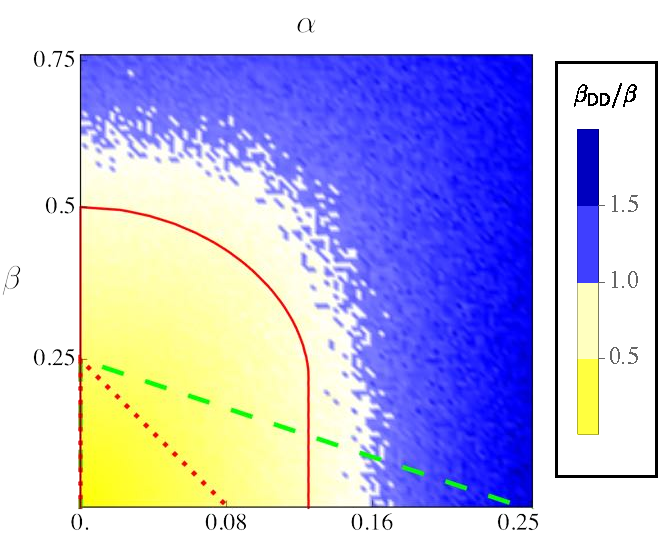
\includegraphics[width=0.8\linewidth]{pdd-ideal-region}
\caption{The noise reduction ratio $\beta_\sDD/\beta$ obtained through maximization over random bath operators plotted in the $(\alpha,\beta)$ parameter plane. In comparison, the theoretical boundaries for noise reduction are also plotted, with dotted red line for (\ref{eq:pdd-region-strict}) and solid red line for (\ref{eq:pdd-region}), also with the boundary for the absolute-convergence condition (\ref{dd:PDD-magnus-abs}) in dashed green line. Note the ranges for $\alpha$ and $\beta$ are chosen differently for better visual effect.}
\label{fig:pdd-region}
\end{figure}

As long as the two-component norm of the free evolution Hamiltonian falls in the yellow region on the lower-left corner, the idealist PDD scheme is guaranteed to work, in the sense of reducing the error phase. This reflects the fundamental ``small noise'' assumption of DD. From the numerical results, we learn that the bound by the ``strict condition'' from (\ref{eq:pdd-region-strict}) is too loose compared with the ``approximate condition'' (\ref{eq:pdd-region}), which works surprisingly well in reflecting the true boundary of the noise-reduction region. The faithfulness of the latter bound is particularly striking considering the points beyond the absolute-convergence boundary (above the green dotted line), where our derivation should be unreliable in principle. An explanation is that the absolute-convergence criteria (\ref{dd:PDD-magnus-abs}), sufficient but not necessary, is a loose one and the leading order Magnus series works well beyond the region predicted by this inequality. This piece of evidence boosts our confidence in using the leading order Magnus term as approximation in the following parts of this work. But for safety, the absolute convergence region will also be indicated. 
}



%%%%%%%%%
\subsection{Noisy Gates}
Previously, we treated the DD control gates in an ideal manner, which implies instantaneous and noise-free pulses. In practice, of course, the control gates are neither instantaneous nor noise-free. Hence the analysis for ideal DD cannot be directly carried out.

The effects of quantum noise on the system can be generally modelled with CPTP channels, which need not be unitary. The introduction of non-unitarity is problematic as the error phase, which is used to study the efficacy of DD, can no longer be defined.
However, one may include some ancillary qubits to transform any quantum channel into a unitary evolution over the extended Hilbert space. For the analytical treatment below, we will always assume this dilation for the noisy gates. Hence, we can ascribe Hamiltonian generators for the noisy control gates. 
Such generator can be time-dependent and involves in the term necessary for the control in addition to various sources contributing to the noise. 
Focusing on the $i$th gate-interval,  we can write the total Hamiltonian:
\begin{equation}\label{eq:noisy-Hamiltonian}
 H(t) = H_e + H_c(t), \quad t_{i-1}< t \le t_i,
\end{equation}
where $H_e=H_\rB+H_\rSB$ is the error Hamiltonian between system and bath, $H_c(t)$ is the control Hamiltonian generating the gate $P_i$ .
For the ideal case, $H_c(t) \propto \delta(t-t_i)$, the corresponding time evolution operator is simply $P_i \upe^{-\upi \tau H_e} =P_i \upe^{-\upi \Omega}$. For the noisy case, it is still assumed that the control Hamiltonian will approximately generate the ideal gate:
\begin{equation}\label{eq:Pi_approx}
 P_i \approx\cT_{\leftarrow} \upe^{-\upi \int_{t_{i-1}}^{t_i} H_c(t) \dd t }.
\end{equation}
A similar noise model was considered in Ref.~\!\cite{khodjasteh2007performance} for the case of finite-width rectangle pulses, where $H_c(t)$  is piecewise-constant and the approximation in \Eqref{eq:Pi_approx} is exact.  Our work allows more broader types of noise while focusing on the break-even conditions for the DD sequence. 

Directly solving the DD time evolution by Magnus series from $H(t)$ in \Eqref{eq:noisy-Hamiltonian} will not work as the very large $H_c(t)$ integral in the matrix exponent will break the convergence condition. It is still necessary to separate the ``pure gate'' parts from the ``free evolution'' parts.   We may express the formal solution to unitary time evolution for the $i$th gate interval as:
\begin{equation}
 \wtU(t_i,t_{i-1})
 = P_i \upe^{-\upi \wtO_i}, 
\end{equation}
where the gate-dependent $\wtO_i$ replaces the free evolution generator $\Omega$ for ideal DD. 
We put tildes over operators to signify that the DD control gates are noisy. 
We can split the $P_i$s by defining $P_i=G_{i+1}^\dagger G_{i}$ and then,
\begin{equation}
\begin{aligned}
  \wtU_\rDD= \upe^{-\upi  G_L \wtO_L  G_L^\dagger} \ldots
  \upe^{-\upi G_2 \wtO_2  G_2^\dagger} \upe^{-\upi G_1\wtO_1G_1}\equiv\upe^{-\upi\wtO_\rDD} .
\end{aligned}
\end{equation}
Provided \Eqref{eq:Pi_approx} holds, the $\wtO_i$s are small and we may use the Magnus formula to derive the leading order Magnus series as good approximation to $\wtO_\rDD$.

The overall goal is to figure out the conditions such that the noise-inflicted DD error phase $\wtep \equiv \norm{\wtO_{\rDD,\rSB}}$  is still reduced compared to the bare Hamiltonian error phase $\phi_\rSB = \norm{\Omega_{\rSB}}$. For simplicity, let us employ a single parameter $\eta$, which is defined later,  to quantify the noise strength associated with the gates.  The break-even condition is, in essence, to invert the inequality
\begin{equation}
 \wtep(\phi_\rB,\phi_\rSB,\eta) < \phi_\rSB,
\end{equation} 
and obtain an upper bound on the noise level $\eta<\eta_{\rmax}(\phi_\rB, \phi_\rSB)$.
To achieve this, we need to correctly estimate the DD error phase function $\wtep(\phi_\rB,\phi_\rSB,\eta)$ while also looking for an appropriate definition for the noise strength $\eta$ associated with the gates.  

 In the followings, we will mainly focus on the PDD to derive explicit break even conditions for various noise. But our analysis should be easily generalized to other DD sequences as well.







\subsubsection{Noisy pulses}
If the strength of the control Hamiltonian is much larger than the system bath coupling,   control gates can still be viewed as ``pulses''. In this section we consider noisy pulses, that is 
$H_c(t)\sim \delta(t-t_i)$, but are noisy.
The  time evolution operator for the $i$th gate interval becomes:
\begin{equation}
 \wtU(t_i,t_{i-1}) = \wtP_i \upe^{-\upi \Omega},
\end{equation}
where $\widetilde{P}_i$ is the noisy pulse version for the ideal $P_i$ gate and $\Omega=\tau H_e$ is the free evolution generator.
Let us also associate to $\wtP_i$ a Hermitian generator, which should be dominated by that of an ideal gate in addition to a small noise part:
\begin{equation}\label{eq:pulse-hami}
 \widetilde{P}_i= \exp\left[ -\upi \left( \Omega_{P_i} +  \eta \Gamma_{P_i} \right)  \right],
\end{equation}
where $\Omega_{P_i}$ is responsible for generating the ideal gate $P_i = \exp(-\upi \Omega_{P_i})$ and supported only on the system; and $ \eta \Gamma_{P_i} $ is responsible for the noise and supported on the system-bath-ancilla composite in general. We have introduced the explicit small parameter $\eta$ to facilitate order tracking. For PDD in particular, the sequence comprises only $X$ and $Z$ gates. 
And we may write the noisy $X$ and $Z$ pulses as:
\begin{equation}\label{eq:gatedep-noise}
\widetilde{X} = \upe^{-\upi ( \frac{\pi}{2} \sigma_1 + \eta\Gamma')},\quad
 \widetilde{Z} = \upe^{-\upi ( \frac{\pi}{2} \sigma_3 + \eta\Gamma'')}.
\end{equation}
We further decompose $\Gamma' = \sum_i \sigma_i \otimes B'_i $ and $\Gamma''=\sum_i \sigma_i \otimes B''_i$, with $B'_i$ and $B''_i$ acting on the bath and the potential ancilla space. 
The time evolution for the noisy PDD sequence then becomes
\begin{equation}\label{eq:UPDD-gatedep}
 \begin{aligned}
\wtU_\rDD &=
 \widetilde{Z} \upe^{-\upi \Omega}
 \widetilde{X} \upe^{-\upi \Omega}
 \widetilde{Z} \upe^{-\upi \Omega}
 \widetilde{X} \upe^{-\upi \Omega}\\
 & = \upe^{-\upi  \eta\Gamma_3} \upe^{- \upi\Omega_3}
 \upe^{-\upi  \eta\Gamma_2}  \upe^{-\upi\Omega_2}
\upe^{-\upi  \eta\Gamma_1} \upe^{-\upi\Omega_1}
\upe^{-\upi  \eta\Gamma_0}  \upe^{-\upi \Omega_0},
\end{aligned}
\end{equation}
where we define $\Omega_i\equiv\sigma_i\Omega\sigma_i$ and
$\upe^{-\upi  \eta\Gamma_3}=\wt Z Z$, 
$\upe^{-\upi  \eta\Gamma_2}=Z \wt X Y$,
$\upe^{-\upi  \eta\Gamma_1}=Y \wt Z X$ and 
$\upe^{-\upi  \eta\Gamma_0}=X \wt X$.
By keeping the first order in 
$\eta$, we can derive
\begin{equation}
 \begin{aligned}
  \Gamma_3 &= \sigma_0 \otimes B_0''- \frac{2}{\pi} \sigma_1 \otimes B_2'' 
  +\frac{2}{\pi}  \sigma_2 \otimes B_1'' + \sigma_3 \otimes B_3'',\\
  \Gamma_2 &= \sigma_0 \otimes B_0'- \sigma_1 \otimes B_1'
  +\frac{2}{\pi}  \sigma_2 \otimes B_3' + \frac{2}{\pi} \sigma_3 \otimes B_2',\\
  \Gamma_1 &= \sigma_0 \otimes B_0''+ \frac{2}{\pi} \sigma_1 \otimes B_2'' 
  +\frac{2}{\pi}  \sigma_2 \otimes B_1'' - \sigma_3 \otimes B_3'',\\
  \Gamma_0 &= \sigma_0 \otimes B_0'+ \sigma_1 \otimes B_1'
  +\frac{2}{\pi}  \sigma_2 \otimes B_3' - \frac{2}{\pi} \sigma_3 \otimes B_2'.
 \end{aligned}
\end{equation}
Every term on the exponent in \Eqref{eq:UPDD-gatedep}  is now at least linear in the smallness $\eta$ or $\norm{\Omega}$ and we can apply the Magnus formula to calculate $\widetilde\Omega_\mathrm{PDD}$. 
The first order Magnus term suggests:
\begin{equation}
 \wt\Omega_\rDD\up{1}= \sigma_0 \otimes (4B_0 + 2\eta( B'_0 + B''_0)) 
+ \sigma_2 \otimes \frac{4}{\pi}\eta(B_1''+B_3').
\end{equation}
The term that acts non-trivially on the system is proportional to $B_1''+B_3'$. 
Assuming no particular relation between the $X$ and $Z$ noise,  exact first order decoupling is lost. 
When the gate noise strength $\eta$ is at least of similar size as $\phi_\rSB$---the gate noise is typically stronger than the background noise in many experiments---the first order Magnus term would be of leading order in magnitude. And the error phase after PDD is reduced to a linear multiple in $\eta$. 
 we upper-bound the size of the first order coupling by:
\begin{equation}
 \wt\Phi_\rSB \approx \norm{ \frac{4\eta}{\pi}(B_1''+B_3')} \le \frac{8}{\pi}\eta.
\end{equation}
This results in the first order breakeven condition:
\begin{equation}
 \eta \le \frac{\pi}{8} \phi_\rSB.
\end{equation}
This condition indicates that in order to achieve noise suppression, the gate noise should be bounded by a fraction of the free evolution noise. If any observable improvement from DD is expected, the pulses must be very accurate in the first place.   On the other hand if $\eta\ll \phi_\rSB$, the existence of pulse noise contributes negligibly and the second oder term will be similar to the ideal PDD case. Hence to faithfully approximate the full $\wt\Omega_\rDD$, we may keep every term that is linear in $\eta$ and up to second order in the smallness $\phi_\rB$ or $\phi_\rSB$ (alternatively: second order in $\phi$). Focusing on the interaction part, the result becomes:
\begin{equation}
 \wt\Omega_{\rDD:\rSB} = \mathfrak{D}(\Omega_{\rDD:\rSB}) +\sigma_2 \otimes \frac{4}{\pi}\eta(B_1''+B_3') + \cO(\eta\phi,\phi^3).
\end{equation}
Bounding the resulting error phase and applying triangular inequality, we have the second order break even condition:
\begin{equation}
   \eta \le \frac{\pi}{8} \phi_\rSB - \frac{\pi}{8}\Phi_\rSB^{(\mathrm{ub})}.
\end{equation}
For verification, we numerically simulated PDD with noisy pulses and compare the results with our our break even conditions in \Figref{fig:pdd-noisy-pulse}. 
Specifically, for each fixed tuple of parameters $(\phi_\rB,\phi_\rSB,\eta)$, we randomly generate 300 sets of the Hermitian matrices $\{\Omega,\Gamma',\Gamma''\}$
satisfying the given parameters over a uniform distribution. Noisy PDD is simulated for each particular set of  bare Hamiltonian and noisy pulses; the noise reduction ratio $\wt\Phi_\rSB/\phi_\rSB$ is obtained and numerically maximized for the fixed $(\phi_\rB,\phi_\rSB,\eta)$. 
We used two figures to visualize the effect of noisy pulses. First is the deformation---or shrinking to be exact---of the noise removal region in the $(\phi_\rB,\phi_\rSB)$ phase diagram. Second is the dependence between the maximally allowed noise versus the free-evolution noise. From the figure we can see that our first order condition works well as long as the noise parameter $(\phi_\rB,\phi_\rSB)$ is weak and the second order condition is more universally applicable for a wider range of conditions.



 \begin{figure}
 \centering
 \begin{subfigure}{0.8\linewidth}
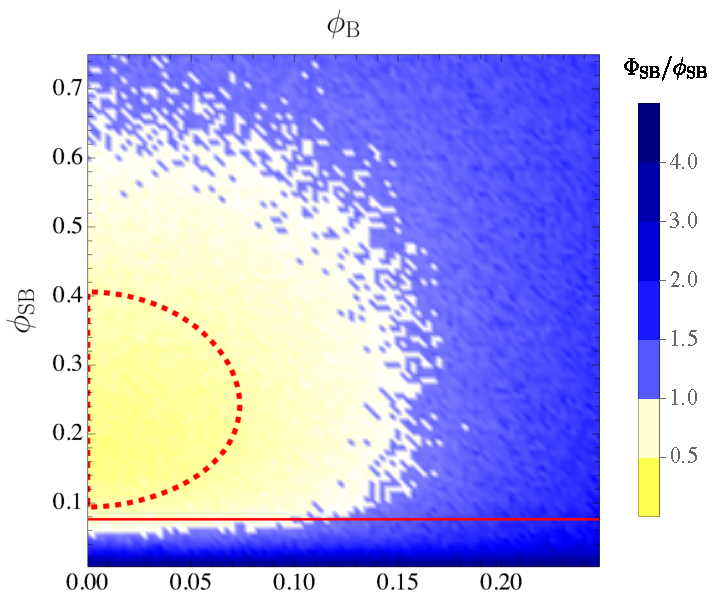
\includegraphics[height=0.8\linewidth]{pdd-noisypulse1}
\caption{$\eta =0.03$.}
\end{subfigure}
\\
\begin{subfigure}{0.8\linewidth}
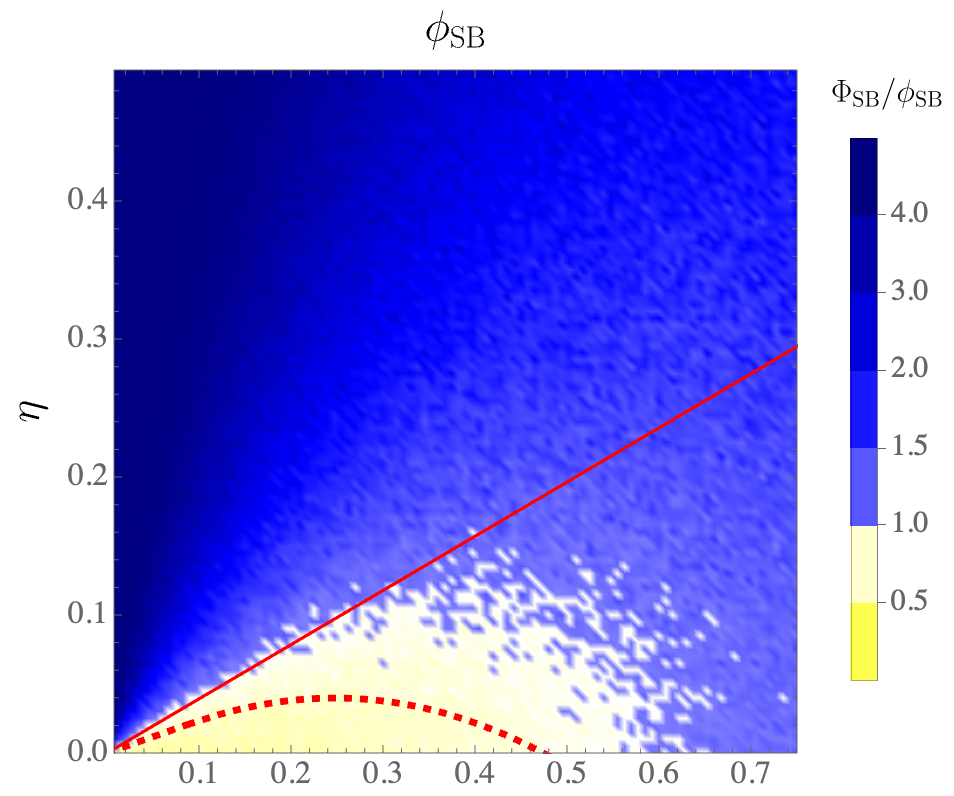
\includegraphics[height=0.8\linewidth]{pdd-noisypulse2}
\caption{$\phi_\rB =0.05$.}
\end{subfigure}
\caption{The maximal noise reduction ratio for the noisy PDD. A point is colored yellow if the noise is reduced after PDD.  The first order condition is indicated with the red solid line while the second order condition is indicated with the red dashed line. }
\label{fig:pdd-noisy-pulse}
\end{figure}



We now examine the special scenario where the first order decoupling is exact, which requires $B''_1+B'_3=0$. It can be shown that this condition actually corresponds to a ``weakly gate-dependent'' noise model:
\begin{equation}\label{eq:gateindep1}
 \wtP_i = P_i \upe^{-\upi \eta \Gamma + \cO(\eta^2)},\ \forall i.
\end{equation}
For the most generic noisy pulses, we can write introduce the gate-noise decomposition $\wtP_i = P_i \upe^{-\upi \eta \Gamma_i}$. The weak gate-dependence assumption is demanding that the variance in $\Gamma_i$  
is at most on the order of the smallness parameter $\eta$.
 That is, the dependence of the noise on the gate is weak. If this condition is 
 satisfied, then the time evolution readily reduces to the ideal DD case by replacing $\Omega=\tau H$ for free evolution with an effective Hamiltonian $\wtO$ such that
\begin{equation}
\upe^{-\upi \wtO}=\upe^{-\upi \eta \Gamma}\upe^{-\upi \Omega}.
\end{equation}
Since $\Gamma$ and $\Omega$ are both small, as required for DD to work,
one may invoke the BCH formula to get $\wtO$ as a series of nested commutators. 
The already established map $\Omega\to \Omega_{\rDD}$ for the idea-pulse DD sequence can then be reused to estimate $\Omega_{\rDD}$
Naturally, we recover exact first order decoupling for PDD. To derive the break-even condition for such weakly gate-dependent noise, 
we retain the BCH series to the second order term, and then apply triangular inequality to derive the upper bounds for $(\widetilde\phi_\rB,\widetilde{\phi}_\rSB) \equiv( \norm{\wtO_\rB}, \norm{\wtO_\rSB})$:
\begin{equation}\label{eq:comb-bound}
\left\{
\begin{aligned}
 \widetilde\phi_\rB &\lesssim (\eta + \phi_\rB)(1+\eta + \phi_\rSB) \equiv \widetilde\phi_\rB^{(\mathrm{ub})}\\
 \widetilde\phi_\rSB &\lesssim (\eta + \phi_\rSB) (1+\eta + \phi_\rB)\equiv \widetilde\phi_\rSB^{(\mathrm{ub})}
\end{aligned}
\right..
\end{equation}
With this, we can bound the error phase relevant for this noisy-pulse situation under the different schemes by replacing $\phi_\rB$ and $\phi_\rSB$ for the ideal case with their noisy upper bounds: 
\begin{equation}
 \widetilde\Phi_\rSB \le \Phi_\rSB(\widetilde\phi_\rB^{(\mathrm{ub})}  ,\widetilde\phi_\rSB^{(\mathrm{ub})} ) < \phi_\rSB.
\end{equation}
Further bounding the right hand side by $\phi_\rSB$ then gives us the condition for the break-even points.

The above analysis is generic and applies to all DD schemes with gate-independent noise. 
The resulting bound is general, but could be suboptimal for a specific DD scheme and a specific type of pulse imperfection. Below, we examine a concrete examples of imperfections  for PDD: 
global unitary error in the control gates,  which results in the noisy pulse 
\begin{equation}
\widetilde P_i=P_i\upe^{-\upi \bm{\theta}\cdot\bm\sigma},\ \forall i.
\end{equation}
We use the notation $\bm\sigma=(\sigma_1,\sigma_2,\sigma_3)$, and $\bm\theta\equiv (\theta_1,\theta_2,\theta_3)$ with $\theta_i$ real constants---taken as small for weak noise---that parameterize the unitary error.  This can arise from, for example, a systematic calibration error in the pulse control leading to a consistent over or under rotation. In this situation, $\Gamma\equiv \bm\theta\cdot\bm\sigma$ acts only on the system and does not have a pure bath term. In the appendix, we derive an tighter bound:
\begin{equation}\label{eq:eff-Hami-tcp}
\left\{
\begin{aligned}
\widetilde{\phi}_\rB &\le \phi_\rB + \frac{1}{3}\theta  \phi^2_\rSB  \\
\widetilde{\phi}_\rSB &\le \phi_\rSB +  \theta^2  \phi_\rSB  \\
\end{aligned}    \right.,
\end{equation}
where $\theta \equiv \norm{\bm \theta}$ is the rotation angle associated with the gate error.
Assuming the noise to be small, we may only use the leading order 
approximation, which is by itself accurate to the second order. 
Substituting the upper bounds to  $\Phi_\rSB(\wt\phi_\rB,\wt\phi_\rSB)$ and keeping the leading order terms,  we can predict the following simplified bound for PDD:
\begin{equation}\label{eq:npdd-bound-simple}
2\phi_\rB^2 + \frac{(\theta+\phi_\rSB)^4}{4\phi_\rSB^2}\le \frac{1}{16},
\end{equation}
From this inequality, the globally maximally allowed $\theta$ can be found at $\phi_\rB=0$, $\phi_\rSB=1/8$ with
$\theta_\mathrm{max}= 1/8$. Furthermore, we can solve for $\theta$ in terms of $\phi_\rB$ and $\phi_\rSB$ to arrive at the noise threshold for the rotation angle:
\begin{equation}\label{eq:npdd-err-thres}
    \theta \le (1-32\phi_\rB ^2)^{\frac{1}{4}} \sqrt{\frac{\phi_\rSB}{2} }-\phi_\rSB
    \quad \lesssim \sqrt{\frac{\phi_\rSB}{2}}.
\end{equation}
It states that for the regime where the the free evolution noise is small, gate noise should at most be on the order of the square root of the free evolution noise. This  is quite different from the generic noise case where the upper bound dependence in $\phi_\rSB$ is linear. 


\subsection{finite-width pulses with unitary error}
For the noisy gates, 
we have the time-evolution operator
\begin{equation}
 \wtP_{\sigma_\alpha} =\exp\left[{-\upi \left(\frac{\pi}{2}\sigma_\alpha + \frac{1}{2}\bm \theta_\alpha\cdot \bm \sigma
 + r \Omega
 \right)}\right],  \ \alpha=1,3.
\end{equation}



\newpage
%%%%%%%%%%%%%%%%%%%%%%%%%%%%%
%%%%%%%%%%%%%%%%%%%%%%%%%%%%%
\section{Scaling up protection -- the accuracy threshold}\label{sec:threshold}
\blue{(Generalization of the previous PDD section; CDD content from Secs.~IVA-D of draft by Jiaan \& Xiansong. The main goal here is to show that an accuracy threshold for DD, under the CDD scheme for scaling up, fails to exist. This means that there is a maximum level for CDD, beyond which further levels only make things worse. To discuss the differences from using different measures.)}
We can distinguish between two operational considerations: to preserve states in a quantum memory (no computational gates), or to reduce noise in the course of carrying out a quantum computation. In the memory setting, the goal is to preserve the quantum informational state for some time $T$ without damage. During this time $T$, we can do DD pulses, and ask if the noise at the end of each complete DD sequence is lower than the noise over the same time period if there were no DD pulses. In other words, for DD to work well, we require
\begin{equation}
\textrm{Memory setting:}\quad \epsilon_\mathrm{DD}<\epsilon(L),
\end{equation}
where $\epsilon_\mathrm{DD}$ quantifies the noise after the DD sequence, while $\epsilon(L)$ is the noise after bare evolution for the time taken for the $L$ DD pulses to be applied.
In the computational setting, the comparison of with and without DD is different. With DD, computational gates can only be applied at the completion of each iteration of the DD sequence, as opposed to every time step without DD. The condition for DD to be effective in this case is then
\begin{equation}\label{eq:cond}
\textrm{Computational setting:}\quad\epsilon_\mathrm{DD}<\epsilon(1),
\end{equation}
where $\epsilon(1)$ is the noise after bare evolution for a single time step. 

\begin{figure}[htbp]
 \centering
 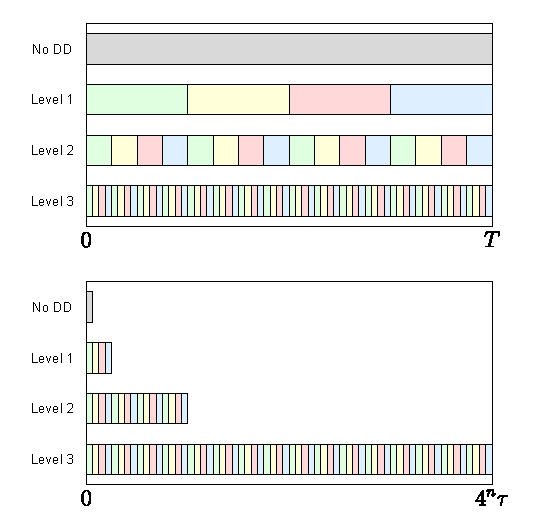
\includegraphics[width=\linewidth]{memory-vs-computation}
 \caption{\blue{An illustration of the CDD time evolution maps under increasing concatenation levels.  We compare the quantum memory setting (above) to the quantum computation setting (under).}}
 \label{fig:memvscom}
\end{figure}

\blue{These two perspectives result in very different overall decoupling strategies. Especially if one is using CDD to ``scale up protection''. As illustrated in Fig.~\ref{fig:memvscom}, for the quantum memory setting, as total time is fixed $T$, one only need to come up with finer and finer slicing of the time evolution pieces; but for the quantum computation setting, one need to join the DD control gates to form a dilated time evolution map. The past papers in favor of CDD had taken the former perspective. It is undeniable that with finer and finer slicing of time evolution, one gets better and better performance. But this picture has some series drawbacks. First the total evolution time $T$ is typically unknown, even for quantum memory. Hence there is no way of knowing in advance which gate to perform at what time. Second, there exists a minimal switch/cool-down time between consecutive gates due to 
technological limitations. Hence it is impractical to arbitrarily suppress noise by increasing concatenation level. 
} 

In our work, we focus on the computational setting, the more stringent one among the two, though it is straightforward to modify our analysis for the memory case. As we will see, Condition \eqref{eq:cond} will yield a requirement on the noise parameters characterizing the noise in the system and the DD pulses. We refer to that requirement as the ``break-even point" for DD, borrowing terminology from quantum error correction and fault-tolerant quantum computing.\red{ (There was a comment in the .tex file that some past papers have analyzed the memory case. What are those papers? Do you just mean the Khodjasteh-Lidar 2007 paper? That paper looks only at imperfections due to finite-width pulses, not control errors as we do here. Their paper hence only has a single-parameter $\ep$, not our two-parameter $\ep$ and $\eta$ situation. In fact, in current experiments $\eta$ is likely the larger problem; memory noise is usually much smaller than gate noise. Or are there other earlier papers?)} \blue{(Yes, that paper in particular. Their conclusion that CDD decouples to order $n$ and dramatically outperforms PDD come from this perspective. Our paper is focused on the quantum computation case which is more practical. See my new added picture \ref{fig:memvscom}). And let me quote their words (bottom left page 10) on how they do the comparison: ``The higher order data for PDD are obtained by simply repeating the basic sequence and shrinking the pulse interval. This is necessary to get the long-term behavior of decoupling. \ldots''  I move this memory/computation argument from the previous  section as it is more appropriate when we discuss the scaling behavior.  ---Jiaan)}

\blue{(To be merged with the new text.) }\gray{The conditions for achieving noise suppression are already derived previously for the idealistic PDD and CDD case.
In general, we find that smaller $(\alpha,\beta)$ values would lead to to better noise suppression rate. Therefore the gates should be performed as frequently as possible. But this may leads to suboptimal outcomes in practice given the extra noise introduced by imperfect gate operations. To study the fault-tolerance of DD, we must account for the additional noise associated with the control gates.}



Next, we turn to the situation of CDD. We can certainly discuss the break-even point for a particular $\CDDn$ sequence, treating it simply as a ``flattened" sequence of pulses, and ask when the error phase after $\CDDn$ is smaller than $\phi_\rSB$ as was done for PDD in the previous section. 
However, what is more interesting is the question of the so-called accuracy threshold for CDD.
As described in the Preliminaries section, CDD tries to achieve better and better noise removal by concatenating the same basic DD scheme---PDD for our discussion here---to higher and higher levels. Here, we are interested in understanding how the noise removal improves as the DD scheme scales up. In fault-tolerant quantum computing, there is the concept of a fault tolerance noise threshold, a strength of the noise below which scaling up the QEC code leads to improved protection against noise, and hence more accurate quantum computation. This threshold is referred to as the accuracy threshold. Here, we ask the analogous question of CDD, whether there is a condition on the noise parameter of the problem such that increasing the CDD level always leads to improved noise removal capabilities. An accuracy threshold for CDD exists if the parameters governing the noise of the situation satisfying a condition $\eta<\eta_0$, such that 
\begin{equation}\label{eq:thresCond}
\Phi_{\mathrm{SB},n+1} < \Phi_{\mathrm{SB},n}\qquad\forall n=1,2,\ldots.
\end{equation}

Below, we examine this for both the ideal CDD case where pulses are perfect, and the noisy CDD case where imperfections in the pulses are allowed.

\newpage
%%%%%%%%%
\subsection{Ideal case}
If a noise threshold indeed exist, then ideal case, where the noise is non-existent, would definitely apply. 
We first consider CDD with perfect pulses. Khodjasteh and Lidar propose in their paper to truncate to th second order term
gave in their paper an estimation of the $\CDDn$ generator as:
\begin{align}\label{eq:cdd-generator-est}
\Omega_{(n)} 
\approx {} & \sigma_0 \otimes 4^n B_0 \notag \\
+\ & \sigma_1 \otimes (-\upi)^{n} 2^{n(n+1)} \ad_{B_0}^{n}(B_1)\\ 
+\ & \sigma_2 \otimes (-\upi)^{n} 2^{n^2} \ad_{B_0}^{n-\!1}( \,[B_0,B_2] - \upi \{B_1,B_3\} \,). \notag
\end{align} 
It is shown in the appendix \ref{app:CDD} that the above expression indeed captures the leading order behavior of $\Omega_{(n)}$. Different from the leading order term in the Magnus series, the leading order ``behavior'' is manifested separately for the pure bath part and the interaction part.  As mentioned in the Preliminaries section, $\CDDn$ achieves $n$th-order decoupling.  From the leading order expression, we see it is indeed so as the interaction part is of $(n+1)$th order.
From \Eqref{eq:cdd-generator-est}, we can 
estimate $\Phi_{\mathrm{B},n} \simeq 4^n\phi_\rB$ and derive an upper bound for for the error phase:
\begin{equation}
\Phi_{\mathrm{SB},n} \lesssim \,
2^{n(n+2)} \phi_\rB^{n}\,\phi_\rSB \,f_n\!\left(\frac{\phi_\rSB}{\phi_\rB}\right),
 % \left\{
 % \begin{aligned}
 % 2^n, && \frac{\phi_\rSB}{\phi_\rB} \le \sqrt{4^n-1}. \\
 % \sqrt{1+\frac{1}{4}\left(\frac{4^n-1}{\phi_\rSB/\phi_\rB}+\phi_\rSB/\phi_\rB\right)^2}, && \frac{\phi_\rSB}{\phi_\rB} > \sqrt{4^n-1}.
 % \end{aligned}
 % \right.
\end{equation}
where we define the piece-wise function:
\begin{equation}
 f_n(x) =\left\{
 \begin{aligned}
 &1, && x \le  \sqrt{4^n-1}, \\
 &\frac{1}{2^n} \sqrt{\left(\frac{4^n-1}{2x}+\frac{x}{2}\right)^2+1}, &&
 x > \sqrt{4^n-1}.
 \end{aligned}
 \right.
\end{equation}

to remind the reader, $\phi_\rB\equiv\phi_\rB(\tau_0)\equiv\tau_0\Vert \HB\Vert$, and $\phi_\rSB\equiv\phi_\rSB(\tau_0)\equiv\tau_0\Vert\HSB\Vert$, noting the dependence of both quantities on $\tau_0$, the time interval between two consecutive pulses in the CDD sequence. \red{(To reconsider: We need both an upper and lower bound for $\Phi_{\mathrm{SB},n}$, which we have from the estimator [Eq.~\eqref{eq:lu}]. For use in Eq.~\eqref{eq:thresCond}, we should have the lower bound on the RHS of that condition, and upper bound expression on the LHS, for a sufficient condition.) } As mentioned in the Preliminaries section, $\CDDn$ achieves $n$th-order decoupling. This can be understood from the error phase expression: $\Phi_{\mathrm{SB},n}$ after $\CDDn$ is of order $\phi^{n+1}$, for $\phi\sim\phi_\rB, \phi_\rSB$. That $\phi_\rB$ enters the error phase should again be of no surprise---as in the PDD case, $\phi_\rB$ determines how quickly the noise seen by the system evolves, and hence affects the efficacy of DD which does a good elimination of the noise only when the noise remains nearly unchanged for the full DD sequence. 

What is perhaps more surprising is the appearance of the $2^{n(n+2)}$ factor in $\Phi_{\mathrm{SB},n}$, a new feature in the CDD case \red{(Do these factors also appear in the Khodjasteh-Lidar analysis? Please check and put in a sentence about this.)}. For fixed $\tau_0\equiv \tau$ as $n$ increases (e.g., if $\tau$ is the experimental limit for the switch time between consecutive pulses), such factors mean that the error phase eventually increases for large enough $n$: The exponentially decreasing $\phi^n$ factor is eventually overcome by the super-exponentially increasing $2^{n^2}$ factor. This means there is no accuracy threshold, i.e., there is no level of noise that is weak enough such that $\Phi_{\mathrm{SB},n+1}\leq\Phi_{\mathrm{SB},n}$ for all $n$. Instead, there is an maximal useful level of concatenation level, beyond which further concatenation actually increases the noise seen by the system. Fig.~\ref{fig:estimator-size} plots this situation of fixed $\tau_0$, for increasing concatenation level $n$. We observe the initial decrease of $\Phi_{\mathrm{SB},n}$ as $n$ increases, but this turns around eventually. 

\begin{figure}
    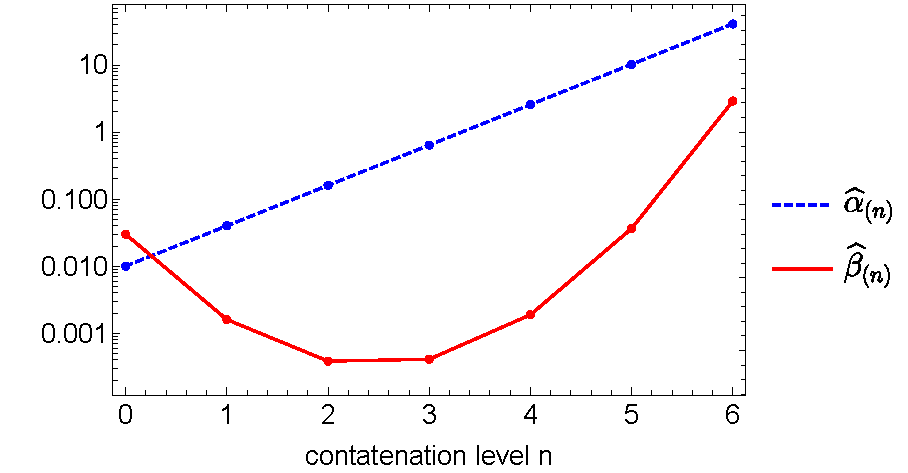
\includegraphics[width=\linewidth]{cdd-estimator}
    \caption{The error phase $\phi_{\rSB,n}$ as a function of concatenation level $n$. 
    The thin color lines are obtained from numerically simulating $\CDDn$ with randomly generated bare Hamiltonian operators satisfying $\phi_\rB=\phi_\rSB=0.001$. The blue dashed line is our theoretical upper bound. For this configuration, we set the maximal concatenation level at 4.}
    \label{fig:estimator-size}
\end{figure}

\red{(To reconsider with my lower/upper bound comment above.) }
For higher concatenation level to make sense, increasing concatenation level should decrease the error phase. To derive a sufficient condition of it, we examine the recursive relation between concatenation 
levels, which suggests 
\begin{equation}
\begin{aligned}
 B_{n+1,0} &= 4  B_{n,0}\\
 B_{n+1,1} & = -4\upi [B_{n,0}, B_{n,1} ]\\
 B_{n+1,2} & = -2\upi [B_{n,0}, B_{n,1} ]\\
  B_{n+1,3} &=0
\end{aligned}
\end{equation}
For both $B_1$ and $B_2$ to decrease in size, it suffice to require the map 
$-4\upi [B_{n,0},\cdot]$ a contraction map. 
By requiring its norm to be smaller than 1, we obtain the bound for the maximal concatenation level:
\begin{equation}\label{eq:cdd-max-level}
n_{\max}\le \lceil-\log_4(\phi_\rB)-3/2\rceil,
\end{equation}
where $\lceil\cdot\rceil$ is the ceiling operator.

Note that the existence of a maximal useful concatenation level does not technically contradict the statement that 
higher-order decoupling is achieved by higher level CDD. Using decoupling order to quantify the degree of noise removal requires, in the first place, the convergence of the Magnus series, so that the $(n+1)$th- and higher-order terms in the series are a small correction to the first $n$ terms. However, if the DD scheme is designed such that the total time for the sequence grows exponentially with $n$, as is the case for CDD if $\tau_0$ is fixed as $n$ increases, eventually, we exceed the convergence criterion and the decoupling order stops being a reasonable indicator of successful noise removal. 

We can, however, analyze a different situation: to have fixed $\tau_n\equiv T$, so that the CDD sequence takes the same amount of time, regardless of $n$. This requires $\tau_0=\frac{T}{4^n}$ for each $n$, so that the pulses are applied at shorter and shorter time intervals as the concatenation level increases. This can be the practical choice if one is doing computation where computational gates, which can only be applied at the end of a complete DD sequence in order to not interfere with the noise averaging process, have to be applied at a particular clock rate. Increasing $n$ to increase the noise removal capabilities must not increase the total time taken for the DD sequence. This requires, of course, the ability to do faster and faster pulse switching.

In this case, it is more illuminating to make use of $\tau_0\Vert \HB\Vert$ and $\tau_0\Vert\HSB\Vert$, in place of $\phi_\rB$ and $\phi_\rSB$, in our estimate of the CDD error phases, so that that the $n$ dependence in $\tau_0$ is explicit. \red{(I suggest we analyze this case as well, to see if an accuracy threshold exists. Jiaan - could you take a quick look at this?)}
Eventually, of course, this becomes limited by the technological---not fundamental---constraint of how fast we can switch between pulses, and thus how short $\tau_0$ can be in an experiment.


%%%%%%%%%
\subsection{Noisy pulses}
\red{(To add.)}

%%%%%%%%%

\red{(To add.)}


%%%%%%%%%%%%%%%%%%%%%%%%%%%%%
%%%%%%%%%%%%%%%%%%%%%%%%%%%%%
\section{Conclusion}
\blue{(To come.)}




%%%%%%%%%%%%%%%%%%%%%%%%%%%%%
%%%%%%%%%%%%%%%%%%%%%%%%%%%%%
\acknowledgments
\blue{(Acknowledge Gu Yanwu, Jonas Tan, and Ryan Tiew, who did some of the first calculations of the breakeven points for PDD. Yanwu should be asked if he wants to be a co-author.)}



\appendix
%%%%%%%%%%%%%%%%%%%%%%%%%%%%%
%%%%%%%%%%%%%%%%%%%%%%%%%%%%%
\section{Analyzing $\CDDn$}\label{app:CDD}
\blue{(To be edited.)}
\gray{
It was suggested by the authors of CDD that the decoupling order for $\mathrm{CDD}_n$  is $n$ \cite{khodjasteh2005fault}. This statement is correct, but their proof is logically flawed. Given its importance, here we explain why the original proof is insufficient and  provide a rigorous proof for the decoupling order.


For the generic $\mathrm{CDD}_n$, it is infeasible to flatten out the gates and calculate the combined Magnus series directly. 
Instead it is easier to study the iteration map 
\begin{equation}\label{eq:CDD-update}
    \Omega_{(n)} = \Opdd(\Omega_{(n-1)}) = \sum_{m=1}^\infty \Opdd\up{m}(\Omega_{(n-1)}),
\end{equation}
where the update map $\Opdd$ is defined in \Eqref{eq:PDD-update}.
Backtracking the map from level $n$ to level $0$, we have
$\Omega_{(n)} = \Opdd\circ \cdots \circ \Opdd(\Omega)
\equiv(\Opdd)^n(\Omega)$.
In the end, the effective Hamiltonian $\Omega_{(n)}$ can be expanded as:
\begin{equation}\label{eq:CDD-magnus}
    \Omega_{(n)} =\sum_{m=1}^\infty \Omega_{(n)}\up{m}(\Omega),
\end{equation}
where $\Omega_{(n)}\up{m}$, with the size of  $\cO(\norm{\Omega}^m)$, is the $m$th order Magnus term in $\Omega$ . Notice that this series is different from the series in \Eqref{eq:CDD-update}, where
each $\Opdd^{(m)}$ generate the $m$th order Magnus term in $\Omega_{(k-1)}$.


To calculate the leading order Magnus term in $\Omega$, we do not directly solve $\Omega_{(n)}$ but instead constructing an estimator $\Ohat_{(n)}$ which is easier to solve. 
Formally we have an estimator-error pair $(\Ohat_{(n)},\delta\Omega_{(n)})$ such that
\begin{equation}\label{eq:est+err}
    \Omega_{(n)} = \Ohat_{(n)} + \delta\Omega_{(n)}.
\end{equation}
The estimator $\Ohat_{(n)}$  is faithful if it captures the leading order behavior of $\Omega_{(n)}$. This is defined separately for the pure-bath part and the coupling part, as they are of different orders.
In other words, a faithful estimator should contain the first nonzero pure-bath part and the first nonzero coupling part of the series (\ref{eq:CDD-magnus}).
An equivalent statement is that the error must be of higher order than the estimator. To quantify this statement, we take the two-component norm for both 
$\delta\Omega_{(n)}$ and $\Ohat_{(n)}$, and demanding
\begin{equation}
\opnorm{\delta\Omega_{(n)}}\equiv
\begin{pmatrix}
\delta\alpha_{(n)}\\
\delta\beta_{(n)}
\end{pmatrix}
\ll 
\opnorm{\Ohat_{(n)}}\equiv\begin{pmatrix}
\widehat\alpha_{(n)}\\
\widehat\beta_{(n)}
\end{pmatrix},
\end{equation}
where the comparison is implied for both components and should be understood by comparing the leading powers of the polynomials in $\alpha$ and $\beta$. 
In essence, a ``smaller'' polynomial should have a larger leading power and thus is of higher order smallness. 
We refer readers to Appendix~\ref{app:polynomials} for more rigorous descriptions on ordering polynomials by their leading powers.
Furthermore, after taking the two-component norm and applying triangular inequality for \Eqref{eq:est+err}, we find,
\begin{equation}\label{eq:lu}
    \widehat\beta_{(n)}-\delta\beta_{(n)}\le  \beta_{(n)}\le \widehat\beta_{(n)}+\delta\beta_{(n)}.
\end{equation}
According to \Eqref{eq:nth-order-alternative}, the $n$th-order decoupling condition requires $\beta_{(n)}$ to be an $(n+1)$th order polynomial in $\alpha$ and $\beta$. It now suffices to show that \numcircled{1} $\widehat\beta_{(n)}$ is an $(n+1)$th order polynomial and \numcircled{2} the estimator is faithful.

The original CDD paper (Ref.\cite{khodjasteh2005fault}) constructed an estimator by keeping the first two Magnus terms for each iteration step. In
our notation:
\begin{equation}
    \Ohat_{(n)} \equiv (\Opdd\up{1} + \Opdd\up{2}) (\Ohat_{(n-1)}) = \big(\Opdd\up{1} + \Opdd\up{2}\big)^n (\Omega).
\end{equation}
With $\Opdd\up{1}, \Opdd\up{2}$ explicitly defined in \Eqref{eq:PDD-magnus-1} and \Eqref{eq:PDD-magnus-2}, and the starting point $\Ohat_{(0)}\equiv\Omega$,  the estimator can shown to be specified by the formula:
\begin{align}\label{eq:cdd-estimator}
\Ohat_{(n)} 
={} & \sigma_0 \otimes 4^n B_0 \notag \\
+\ & \sigma_1 \otimes (-\upi)^{n} 2^{n(n+1)} \ad_{B_0}^{n}(B_1)\\ 
+\ & \sigma_2 \otimes (-\upi)^{n} 2^{n^2} \ad_{B_0}^{n-\!1}( \,[B_0,B_2] - \upi \{B_1,B_3\} \,). \notag
\end{align} 
After taking the two-component norm of the estimator, we have,
\begin{equation}
\begin{pmatrix}
\widehat\alpha_{(n)}\\
\widehat\beta_{(n)}
\end{pmatrix}
\simeq
\begin{pmatrix}
\alpha\\
\alpha^{n} \beta +\alpha^{n-1} \beta^2
\end{pmatrix},
\end{equation}
where $\simeq$ represents equal the leading powers as described in Appendix~\ref{app:polynomials}. 
This verifies that $\widehat\beta_{(n)}$ is a an $(n+1)$th order polynomial.

To complete the theory, it now remains to show that $\Ohat_{(n)}$ is indeed faithful. For simplicity, we make the recognition $\alpha\simeq\beta\simeq\Dt$.
This change does not affect the criteria for $n$th order decoupling as the polynomial order is unchanged. To show $\delta\alpha_{(n)}$ and $\delta\beta_{(n)}$ are of higher order in $\tau_0$ compared to $\widehat\alpha_{(n)}$ and $\widehat\beta_{(n)}$, we claim that:
\begin{equation}\label{eq:cdd-error-bounds}
\begin{pmatrix}
\delta\alpha_{(n)}\\
\delta\beta_{(n)} 
\end{pmatrix}
\lesssim
\begin{pmatrix}
\Dt^3\\
\Dt^{n+2} 
\end{pmatrix}.
\end{equation}
We prove this assertion by mathematical induction.
At $n=1$,  i.e.\ the PDD sequence, the error comes solely from the Magnus series truncation.
Taking the two-component norm and applying triangular inequality:
\begin{equation}
\opnorm{\delta\Omega_{(1)}}\le\sum_{m=3}^\infty \opnorm{\Omega_{(1)}\up{m}}
\simeq \opnorm{\Omega_{(1)}\up{3}} \lesssim
\begin{pmatrix}
\Dt^3\\
\Dt^3
\end{pmatrix}.
\end{equation}
By definition, the higher level error term $\delta\Omega_{(n+1)}$ can be 
expressed with the lower level functions as:
\begin{multline}\label{eq:error update}
\delta\Omega_{(n+1)} 
=\Opdd(\Omega_{(n)})-(\Opdd\up{1}+\Opdd\up{2})(\Ohat_{(n)})\\
= \Opdd\up{1}(\delta\Omega_{(n)})+ \sum_{m=2}^\infty \Opdd\up{m}(\Omega_{(n)})-\Opdd\up{2}(\Ohat_{(n)}),
\end{multline} 
where we have used the fact that $\Opdd\up{1}$ is a linear map. Assuming  \Eqref{eq:cdd-error-bounds} holds for level $n$, we need to show $\opnorm{\delta\Omega_{(n+1)}}\lesssim(\Dt^3,\Dt^{n+3})$.
The argument in the original CDD paper by Khodjasteh and Lidar for truncating the Magnus series have only showed that the higher order Magnus term is smaller by proving
\begin{equation*}
    \opnorm{ \sum_{m=3}^\infty\Opdd\up{m}(\Ohat_{(n)}) } \ll \opnorm{\Ohat_{(n+1)}}.
\end{equation*}
If we take $\delta\Omega_{(n)}=0$, \Eqref{eq:error update} would identity the l.h.s.\  of above as $\opnorm{\delta \Omega_{n+1}}$, then this inequality would indeed indicate that the error term is of higher order.
However \Eqref{eq:error update} suggests that this argument is not sufficient: as
the estimate error $\delta\Omega_{(n+1)}$ comes not only  from the truncation error of the same level, but also accumulates from the lower level error $\delta\Omega_{(n)}$. 
To properly bound the size of the error term, we take the two-component norm on both sides of \Eqref{eq:error update}:
\begin{equation}
\begin{aligned}\label{eq:cdd-error-3terms}
\opnorm{\delta\Omega_{(n+1)} }
&\lesssim \opnorm{ \Opdd\up{1}(\delta\Omega_{(n)}) } + 
\opnorm{\Opdd\up{3}( \Omega_{(n)})} \\
&+ \opnorm{ \Opdd\up{2}(\Ohat_{(n)}+\delta\Omega_{(n)})-\Opdd\up{2}(\Ohat_{(n)})},
\end{aligned}    
\end{equation}
where the infinite sum of Magnus terms higher than third order is lead by the non-vanishing third order. 
We now examine the size of these terms.
The first term in (\ref{eq:cdd-error-3terms}) is easy,
\begin{equation*}
\opnorm{\Opdd\up{1}(\delta\Omega_{(n)})} = \begin{pmatrix}
4 \delta\alpha_{(n)} \\
0
\end{pmatrix}\simeq
\begin{pmatrix}
\Dt^3 \\
0
\end{pmatrix}.
\end{equation*}
To bound the size of the second term, we make two observations for the PDD Magnus series greater than the third order:
\begin{enumerate}
    \item At least one $B_{i\neq0}$ is involved in the coupling part.
    \item At least two $B_{i\neq 0}$ is involved in pure bath part.  
\end{enumerate}
% That is to say, for $\opnorm{X}=(\alpha,\beta)$, 
% the size of  the $m$th order Magnus term can be estimated by
% \begin{equation}
%     \opnorm{\Opdd\up{m}(X)} \lesssim \begin{pmatrix}
%         \beta^2 (\alpha+\beta)^{m-2} \\
%         \beta (\alpha+\beta)^{m-1}
%     \end{pmatrix}, \quad m\ge3.
% \end{equation}
Therefore, the second term can be bounded by
\begin{equation*}
\opnorm{\Opdd\up{3}(\Omega_{(n)})} 
\lesssim\begin{pmatrix}
\beta_{(n)}^2 (\alpha_{(n)}+\beta_{(n)}) \\
\beta_{(n)} (\alpha_{(n)}+\beta_{(n)})^2
\end{pmatrix}
\simeq \begin{pmatrix}
\Dt^{2n+2}\\
\Dt^{n+3}
\end{pmatrix},
\end{equation*}
where we have used $\alpha_{(n)}\lesssim\widehat\alpha_{(n)}$ and $\beta_{(n)}\lesssim\widehat\beta_{(n)}$ according to the induction hypothesis.
This can be alternatively shown by explicitly calculating the third order Magnus term using \Eqref{eq:Magnus-3rd}. 
To bound the third term in (\ref{eq:cdd-error-3terms}), we can calculate the difference $\Opdd\up{2}(\Ohat+\delta\Omega) - \Opdd\up{2}(\Ohat)$
using the expression for $\Opdd\up{2}$ from \Eqref{eq:PDD-magnus-2}.  In the end,
\begin{equation*}
\begin{split}
&\opnorm[\big]{\Opdd\up{2}(\Ohat+\delta\Omega) - \Opdd\up{2}(\Ohat)} 
\lesssim\begin{pmatrix}
    0\\
    \delta\alpha_{(n)}\delta\beta_{(n)}
\end{pmatrix}\\
&+\begin{pmatrix}
    0\\
    \widehat\beta_{(n)}\delta\alpha_{(n)} + \widehat\alpha_{(n)} \delta\beta_{(n)}
    +\widehat\beta_{(n)} \delta\beta_{(n)} 
\end{pmatrix}\simeq
\begin{pmatrix}
    0\\
    \Dt^{n+3}
\end{pmatrix}.
\end{split}
\end{equation*}
Since all three terms are bounded by $(\tau_0^3, \tau_0^{n+3})^\transpose$, so is their sum. This proves our assertion \Eqref{eq:cdd-error-bounds}. \qed

\smallskip

Having showed its faithfulness, we are now confident in using the estimator \Eqref{eq:CDD-magnus} to study the full $\Omega_{(n)}$ of $\mathrm{CDD}_n$. In particular, we have $\alpha_{(n)}\approx\widehat\alpha_{(n)}=4^n \alpha$ and
$\beta_{(n)}\approx\widehat{\beta}_{(n)}$.
Similar as the PDD case, we can derive a strict bound and an approximate bound. For the strict bound, we have
\begin{equation}\label{eq:cdd-errph-bound1}
\begin{aligned}
\widehat{\beta}_{(n)} &\le   2^{n(n+1)}\norm{\ad_{B_0}^{n}(B_1)} \\
&\quad + 2^{n^2} 
\norm{\ad_{B_0}^{n-\!1}([B_0,B_2] - \upi \{B_1,B_3\})}\\
&\le  2^{n(n+1)}\alpha^{n-1}\beta (2^n \alpha+ \alpha + \beta).
\end{aligned}
\end{equation}
}




%%%%%%%%%%%%%%%%%%%%%%%%%%%%%
%%%%%%%%%%%%%%%%%%%%%%%%%%%%%
\bibliography{references}




%%%%%%%%%%%%%%%%%%%%%%%%%%%%%
%%%%%%%%%%%%%%%%%%%%%%%%%%%%%
\appendix


\end{document}
